\documentclass[t]{beamer}

\usepackage{biblatex}
\usepackage{algorithm}
\usepackage{src/templates/algorithmicx/algpseudocode}

\setbeamerfont{footnote}{size=\tiny}

\input{header-presentation}
\title[FPGA for ENC!]{Investigating the Mapping of a Reconfigurable Cryptography Engine on a Zedboard}
\author[bobzhou@bu.edu]{by Boyou Zhou,\\Manuel Egele, Ajay Joshi}
\date[\today]{\today}

\begin{document}
\maketitle

\section*{FPGA for Encryption!}

\section{Intro: Why FPGA?}

\begin{frame}{What is ASIC, FPGA and GPP?}
    \begin{block}{ASIC}
        \begin{itemize}
            \item Application Specific Integrated Circuit
            \item Performance: Best, Cost: Highest, Time to Market: Slowest
        \end{itemize}
    \end{block}
    \begin{block}{FPGA}
        \begin{itemize}
            \item Field Programmable Gate Array
            \item Performance: Good, Cost: Normal, Time to Market: Normal 
        \end{itemize}
    \end{block}
    \begin{block}{GPP}
       \begin{itemize}
            \item General Purpose Processor
            \item Performance: Worst, Cost: Lowest, Time to Market: Fastest
       \end{itemize} 
    \end{block}
\end{frame}

\begin{frame}{Performance Comparison Between GPP, FPGA, and ASIC}
    \begin{figure}
        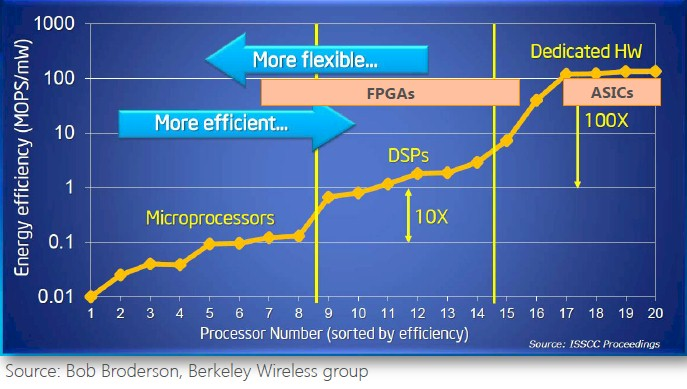
\includegraphics[width=3in]{img/microsoft-fpga-vs-cpu-vs-asic.png}
        \caption{FPGA, FPGA, and ASIC comparison from Microsoft\footcite{http://www.theplatform.net/2015/03/30/why-intel-might-buy-fpga-maker-altera}}
        \label{fig:performance-comparison}
    \end{figure}
\end{frame}

\begin{frame}{IoT Trend}
	\begin{figure}
        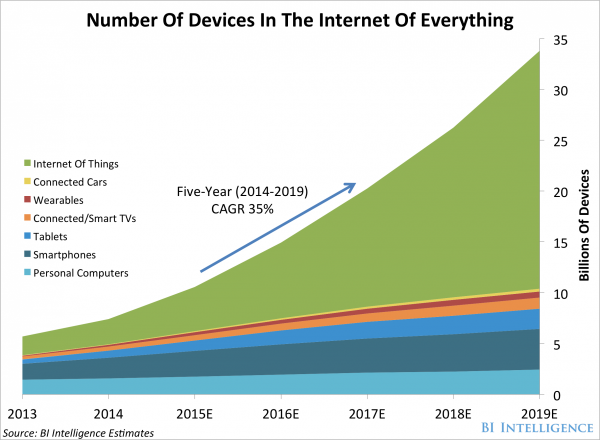
\includegraphics[width=2.5in]{img/iot_trend.png}
		\caption{Iot Trend\footcite{http://www.ironpaper.com/webintel/articles/internet-things-market-statistics-2015}}
		\label{fig:Iot_trend}
	\end{figure}
\end{frame}

\begin{frame}{Architecture}
	\begin{figure}
        \includegraphics[width=2.5in]{img/.png}
		\caption{Iot Trend\footcite{http://www.ironpaper.com/webintel/articles/internet-things-market-statistics-2015}}
		\label{fig:Iot_trend}
	\end{figure}
\end{frame}


\section{Main Work: Use FPGA for Bing}
\begin{frame}{Resolved Problems}
    \begin{block}{Resolved Problems}
        \begin{itemize}
            \item {\tt{Homogeneity Design}} \\
            Homogeneity design reduces management issues and provide consistent platform to
            rely on.
            \item {\tt{Processing Speed}} \\
            Datacenter requests for extreme speed, which CPUs do not provide. 
        \end{itemize}
    \end{block}
\end{frame}


\section{Conclusion}
\begin{frame}{Conclusion}
    \begin{itemize}
        \item They do not have partial reconfiguration.
        \item $95\%$ boost
    \end{itemize}
\end{frame}

\end{document}
